\documentclass{beamer}
\usetheme{Antibes}
\usepackage{xcolor, colortbl}
\usepackage{algorithm}
\usepackage{algpseudocode}
\usepackage{textcomp}
\usepackage{listings}
\usepackage{hyperref}
\usepackage{alltt}
\usepackage{tikz}
\usepackage{framed}
\usepackage{marvosym}
\usepackage{wasysym}
\usepackage{marvosym}
\usepackage{crayola}
\usepackage{mathpartir}
\usepackage{tabularx}
\usepackage[belowskip=-15pt,aboveskip=0pt]{caption}
\usepackage[skins]{tcolorbox}
\usepackage{multicol}
\usetikzlibrary{positioning,shapes,arrows, backgrounds, fit, shadows, automata}
\usetikzlibrary{decorations.markings, calc}
%\usepackage{wasysym}
%\usepackage{marvosym}
\setbeamertemplate{footline}[frame number]
%\usecolortheme{fly}
\usefonttheme{serif}

\title[Sujit]{Lexical Analysis \\
Programming Languages}
\author{Sujit Kumar Chakrabarti}
\institute{IIITB}
\date{}


\definecolor{lightblue}{rgb}{0.8,0.93,1.0} % color values Red, Green, Blue
\definecolor{darkblue}{rgb}{0.4,0.3,1.0} % color values Red, Green, Blue
\definecolor{Blue}{rgb}{0,0,1.0} % color values Red, Green, Blue
\definecolor{darkgreen}{rgb}{0,0.7,0.2} % color values Red, Green, Blue
\definecolor{Red}{rgb}{1,0,0} % color values Red, Green, Blue
\definecolor{Pink}{rgb}{0.7,0,0.2}
\definecolor{links}{HTML}{2A1B81}
\definecolor{mydarkgreen}{HTML}{126215}
\newcommand{\highlight}[1]{{\color{Red}(#1)}}

\newcommand{\myheader}[1]{
	{\color{darkblue}
		\begin{Large}
			\begin{center}
				{#1}
			\end{center}
		\end{Large}
	}
}
\newcommand{\myminorheader}[1]{
	{\color{BrickRed}
		\begin{Large}
			{\fontfamily{\sfdefault}\selectfont\textbf{#1}}
		\end{Large}
	}
}

\newcommand{\kcend}[0]{\begin{center}

\begin{tikzpicture}
\node[rectangle, draw=Red, fill=Red, minimum height=0.25cm]{};
\end{tikzpicture}
\end{center}
}
\tikzstyle{bb}=[%
      rectangle, draw=black, thick, fill=OliveGreen!30, drop shadow, align=center,
      text ragged, minimum height=2em, minimum width=2em, inner sep=6pt
]

\tikzstyle{inv}=[%
      rectangle, draw=none,  align=center,
      text ragged, minimum height=2em, minimum width=2em, align=center, inner sep=6pt
]

\tikzstyle{db}=[%
      ellipse, draw=black, thick, fill=pink, drop shadow, align=center,
      text ragged, minimum height=2em, inner sep=6pt
]

\tikzstyle{jn}=[%
      inner sep=0cm, outer sep=0cm
]

\tikzstyle{io}=[%
      trapezium, trapezium left angle=60, trapezium right angle=120, draw=black, thick, fill=brown, drop shadow,
      text ragged, minimum height=2em, minimum width=2em, inner sep=6pt, align=center
]

\tikzstyle{glio}=[%
      trapezium, trapezium left angle=60, trapezium right angle=120, draw=red, line width = 1mm, fill=brown, drop shadow,
      text ragged, minimum height=2em, minimum width=2em, inner sep=6pt
]
\tikzstyle{gl}=[%
      rectangle, draw=red, line width = 1mm, fill=lightblue, drop shadow,
      text ragged, minimum height=2em, minimum width=2em, inner sep=6pt
]

\tikzstyle{en}=[%
      rectangle, draw=black, thick, fill=none,
      text ragged, minimum height=2em, minimum width=2em, inner sep=6pt
]

\tikzstyle{sh}=[%
      rectangle, draw=gray, thick, fill=none, color = gray,
      text ragged, minimum height=2em, minimum width=2em, inner sep=6pt
]


\lstdefinestyle{javacode}{
	language = Java,
	basicstyle = \ttfamily\scriptsize,
	stringstyle = \ttfamily,
	keywordstyle=\color{Blue}\bfseries,
	identifierstyle=\color{Pink},
	commentstyle=\color{darkgreen},
	frame=single,
	frameround=tttt,
%	numbers=left
	showstringspaces=false
}

\lstdefinestyle{camlcode}{
	language = Caml,
	basicstyle = \scriptsize\ttfamily,
	stringstyle = \color{red}\ttfamily,
	keywordstyle=\color{Blue}\bfseries,
	identifierstyle=\ttfamily,
	frame=single,
	frameround=tttt,
	numbers=none,
	showstringspaces=false,
	escapeinside={(*@}{@*)}
}

\lstdefinestyle{outputcode}{
	language = bash,
	backgroundcolor = \color{black},
	basicstyle = \tiny\ttfamily\color{white},
	stringstyle = \color{red}\ttfamily,
	keywordstyle=\color{white}\bfseries,
	identifierstyle=\ttfamily,
	frameround=tttt,
	numbers=none,
	showstringspaces=false,
	escapeinside={(*@}{@*)}
}

\newtcolorbox{myframe}[2][]{%
  enhanced,colback=white,colframe=black,coltitle=black,
  sharp corners,boxrule=0.4pt,
  fonttitle=\itshape,
  attach boxed title to top left={yshift=-0.3\baselineskip-0.4pt,xshift=2mm},
  boxed title style={tile,size=minimal,left=0.5mm,right=0.5mm,
    colback=white,before upper=\strut},
  title=#2,#1
}

\begin{document}
\maketitle


% frame begin %%%%%%%%%%%%%%%%%%%%%%%%
\begin{frame}{Implementation of Lexical Analysis}
{Finite State Automata}
\myminorheader{Example}

\textbf{ATM:}
\pause
\begin{center}
\resizebox{!}{0.45\textheight}{%
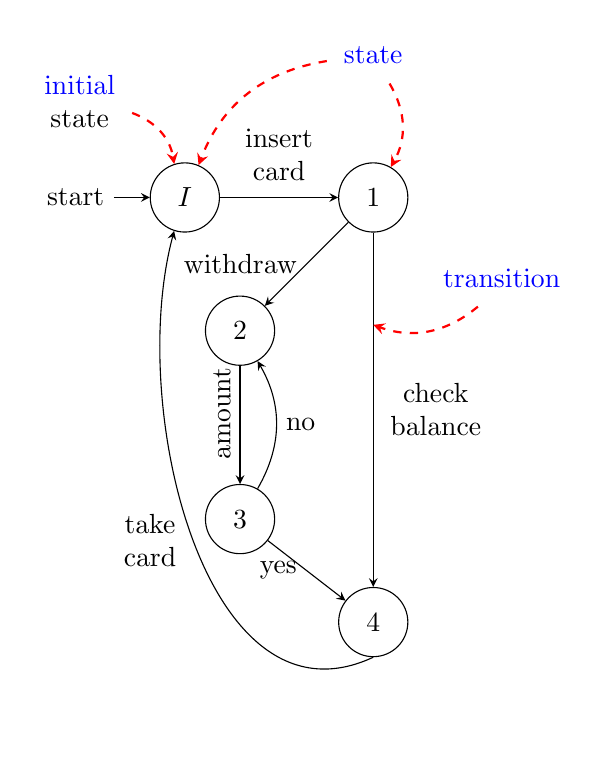
\begin{tikzpicture}[auto,
    ->,
    >=stealth,
    node distance=1.5cm
  ]
    \node[initial, state]   (0)                {$I$};
    \node[state]            (1) [right = of 0] {$1$};
    \node[state]            (2) [below left = of 1] {$2$}; 
    \node[state]            (3) [below      = of 2] {$3$}; 
    \node[state]            (4) [below      = of 1, yshift=-3cm] {$4$}; 
    
    \path (0) edge node [inv, above] {insert \\ card} (1)
          (1) edge node [left] {withdraw} (2)
          (2) edge node [very near end, rotate=90, above right] {amount} (3)
          (3) edge node [left] {yes} (4)
          (3) edge[bend right] node [right] {no} (2)
          (4.south) edge[bend left=40, out=90] node [inv, left] {take \\ card} (0)
    ;
\draw[->] (1) -- node [inv, right] {check \\ balance} (4);

\coordinate (e1) at ($(1)!0.3!(4)$);

\pause

    \node[inv] (l1)[above=1cm of 1] {\color{Blue}state}; 
    \node[inv] (l0)[above left=0.5cm of 0] {\color{Blue}initial \\ state}; 
    \node[inv] (l2)[below right=0.5cm of 1] {\color{Blue}transition}; 

\draw[->, Red, dashed, thick, bend left] (l1) to (1);
\draw[->, Red, dashed, thick, bend right] (l1) to (0);
\draw[->, Red, dashed, thick, bend left] (l0) to (0);
\draw[->, Red, dashed, thick, bend left] (l2) to (e1);
    
  \end{tikzpicture}
}

\end{center}

\pause
\begin{scriptsize}
\begin{itemize}
\item Alphabet $\Sigma$: \{insert card, check balance, no, yes, withdraw, amount, take card \}
\item States, initial state
%\item Accepting/final/terminating states
\item Transitions
\end{itemize}
\end{scriptsize}
\end{frame}
% frame end %%%%%%%%%%%%%%%%%%%%%%%%

% frame begin %%%%%%%%%%%%%%%%%%%%%%%%
\begin{frame}{Implementation of Lexical Analysis}
{Finite State Automata}
\myminorheader{Example}

\textbf{NUMBER:}
\begin{center}
\resizebox{!}{0.5\textheight}{%
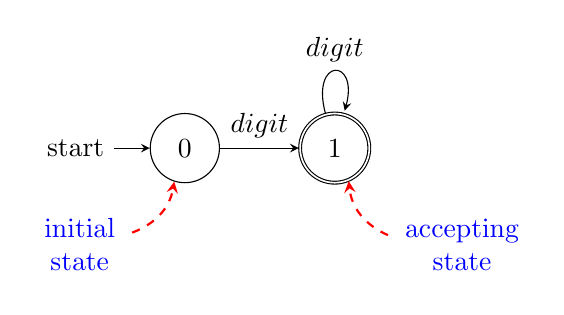
\begin{tikzpicture}[auto,
    ->,
    >=stealth
  ]
    \node[initial, state]   (0)                {$0$};
    \node[state, accepting] (1) [right = of 0] {$1$};
    
    \path (0) edge node {$digit$} (1)
          (1) edge[loop above] node {$digit$} (1)
    ;

\pause    
    \node[inv] (l0)[below left=0.5cm of 0] {\color{Blue}initial \\ \color{Blue}state}; 
    \node[inv] (l1)[below right=0.5cm of 1] {\color{Blue}accepting \\ \color{Blue}state}; 

\draw[->, Red, dashed, thick, bend right] (l0) to (0);
\draw[->, Red, dashed, thick, bend left] (l1) to (1);
  \end{tikzpicture}
}

\end{center}

\end{frame}
% frame end %%%%%%%%%%%%%%%%%%%%%%%%

% frame begin %%%%%%%%%%%%%%%%%%%%%%%%
\begin{frame}{Implementation of Lexical Analysis}
{Finite State Automata as recogniser}

A string can be considered accepted if:
\begin{scriptsize}
\begin{itemize}
\item input pointer has reached the end of the string.
\item machine is in an accepting state.
\end{itemize}
\end{scriptsize}
\pause
A string can be considered rejected if:
\begin{scriptsize}
\begin{itemize}
\item input pointer has reached the end of the string and machine is not in an accepting state.
\item a symbol occurs for which the machine can't make a transition.
\end{itemize}
\end{scriptsize}
\end{frame}
% frame end %%%%%%%%%%%%%%%%%%%%%%%%

% frame begin %%%%%%%%%%%%%%%%%%%%%%%%
\begin{frame}{Implementation of Lexical Analysis}
{Finite State Automata as recogniser}

\myminorheader{Example}

\textbf{DECIMAL NUMBER:}
\begin{center}
\resizebox{!}{0.15\textheight}{%
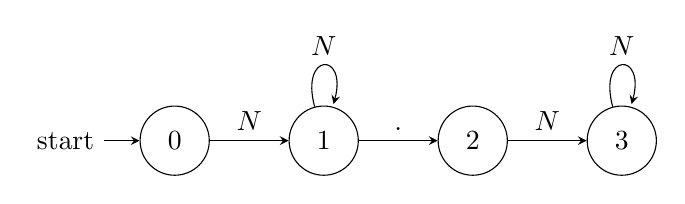
\begin{tikzpicture}[auto,
    ->,
    >=stealth
  ]
    \node[initial, state]   (0)                {$0$};
    \node[state] (1) [right = of 0] {$1$};
    \node[state] (2) [right = of 1] {$2$};
    \node[state] (3) [right = of 2] {$3$};
    
    \path (0) edge node {$N$} (1)
          (1) edge[loop above] node {$N$} (1)
          (1) edge node {$.$} (2)
          (2) edge node {$N$} (3)
          (3) edge[loop above] node {$N$} (3)
    ;
  \end{tikzpicture}
}
\end{center}

\begin{enumerate}
\pause
\item $NN.N$ 
\begin{minipage}{0.5\linewidth}
\begin{flushright}
$0 \xrightarrow{N} 1 \xrightarrow{N} 1  \xrightarrow{.} 2 \xrightarrow{N} 3$ \pause {\color{Green}\checkmark}
\end{flushright}
\end{minipage}

\pause
\item $NN.NN$
\begin{minipage}{0.6\linewidth}
\begin{flushright}
$0 \xrightarrow{N} 1 \xrightarrow{N} 1  \xrightarrow{.} 2 \xrightarrow{N} 3 \xrightarrow{N} 3$ \pause {\color{Green}\checkmark}
\end{flushright}
\end{minipage}

\pause
\item $NN.$
\begin{minipage}{0.5\linewidth}
\begin{flushright}
$0 \xrightarrow{N} 1 \xrightarrow{N} 1  \xrightarrow{.} 2\ \pause {\color{Red}\times}$
\end{flushright}
\end{minipage}

\pause
\item $.N$
\begin{minipage}{0.5\linewidth}
\begin{flushright}
$0 \xrightarrow{.} \pause {\color{Red}\times}$
\end{flushright}
\end{minipage}

\pause
\item $N\alpha$
\begin{minipage}{0.5\linewidth}
\begin{flushright}
$0 \xrightarrow{N} 1 \xrightarrow{\alpha} \pause {\color{Red}\times}$
\end{flushright}
\end{minipage}

\pause
\item $N.N\alpha$
\begin{minipage}{0.5\linewidth}
\begin{flushright}
$0 \xrightarrow{N} 1 \xrightarrow{N} 1  \xrightarrow{.} 2 \xrightarrow{N} 3 \xrightarrow{\alpha} \pause {\color{Red}\times}$
\end{flushright}
\end{minipage}
\end{enumerate}
\end{frame}
% frame end %%%%%%%%%%%%%%%%%%%%%%%%

% frame begin %%%%%%%%%%%%%%%%%%%%%%%%
\begin{frame}{Implementation of Lexical Analysis}
{Finite State Automata as recogniser}

\begin{itemize}
\item Each token class $T$ is represented using an FSA $F$.
\item Acceptance of an input string $i$ by $F$ indicates that $i \in T$.
\item Lexical analyser consumes $i$ and returns $T$.
\end{itemize}

\begin{center}
\resizebox{!}{0.5\textheight}{
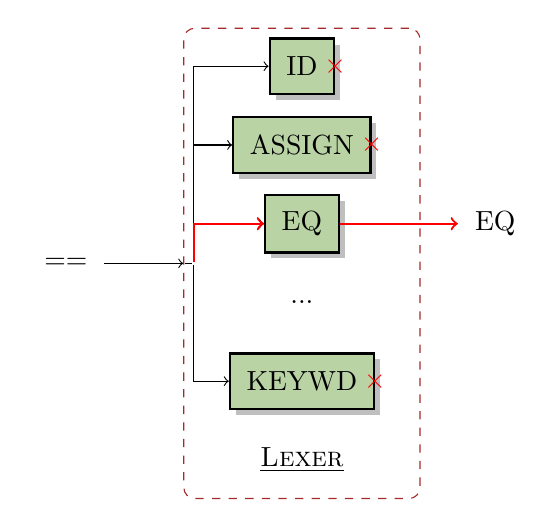
\begin{tikzpicture}
\node[bb](id) {ID};
\node[bb, below of=id](assign) {ASSIGN};
\node[bb, below of=assign](eq) {EQ};
\node[inv, below of=eq](dts) {...};
\node[bb, below of=dts](kwd) {KEYWD};
\node[inv, below of=kwd](lla) {\textsc{\underline{Lexer}}};
\node[draw=Brown, dashed, rounded corners, fit=(id) (kwd) (lla), minimum width=3cm] (la){};



\node[jn] at (la.west) (j1) {};
\node[jn, right=0.1cm of j1]  (j2) {};

\pause
\node[inv, left= of la](i) {$==$};
\draw[->] (i) -- (la);
\pause
\draw[-] (j1) -- (j2);
\draw[->] (j2) |- (kwd);
\draw[->] (j2) |- (id);
\draw[->] (j2) |- (assign);
\draw[->] (j2) |- (eq);

\pause
\node[inv] at (id.east) (fail1){\color{Red}$\times$};
\node[inv] at (assign.east) (fail2){\color{Red}$\times$};
\node[inv] at (eq.east) (pass1){\color{Green}\checkmark};
\node[inv] at (kwd.east) (fail3){\color{Red}$\times$};

\draw[->, thick, Red] (j2) |- (eq);
\node[inv, right=1.5cm of eq] (outp) {EQ};
\draw[->, thick, Red] (eq) -- (outp);
\end{tikzpicture}
}
\end{center}

%\pause
\kcend

\end{frame}
% frame end %%%%%%%%%%%%%%%%%%%%%%%%

%% frame begin %%%%%%%%%%%%%%%%%%%%%%%%
%\begin{frame}{Simulation of FSA}
%\footnotesize
%\begin{algorithmic}[0]
%\Procedure{simFSA}{$M$, $inp$}
%\pause
%  \State $s \gets M.s_0$ \Comment{$M.s_0$ = initial state}
%  \While{there is input left}
%    \State $c \gets$ \Call{nextChar}{}
%    \State $s \gets$ $M$.\Call{move}{$s$, $c$} \Comment{\textsc{move} = transition function}
%    \If{$s$ = \textbf{nil}}
%      \State \textbf{break}
%    \EndIf
%  \EndWhile
%  \If{$s \in M.F$} \Comment{$M.F$ = final states}
%    \State \textbf{return true}
%  \Else
%    \State \textbf{return} \textbf{false}
%  \EndIf
%\EndProcedure
%
%\end{algorithmic}
%\end{frame}
%% frame end %%%%%%%%%%%%%%%%%%%%%%%%


% frame begin %%%%%%%%%%%%%%%%%%%%%%%%
\begin{frame}{Next}

\begin{enumerate}
\item DFA and NFA
\item Implementation of FSAs
\end{enumerate}
\end{frame}
% frame end %%%%%%%%%%%%%%%%%%%%%%%%

\end{document}
